\section{Experimental Results}
\label{chap1:sec:res}

In this section, we present the results of applying the afore-described 
methodology. We use the framework to verify six different isosurface 
extraction codes, namely: VTK Marching Cubes~\cite{lor87},
SnapMC~\cite{Raman:2008:QIM}, Macet~\cite{Dietrich:TVCG:2008},
Dual Contouring~\cite{Ju:2002:DCH:566654.566586}, Afront~\cite{Schreiner06},
and DelIso \cite{Dey07}. All these
implementations are open source and/or publicly 
available. Before presenting the actual results of subjecting these
implementations to the verification process,
we briefly review their salient features.

\subsection{VTK Marching Cubes} Marching Cubes~\cite{lor87} (MC) is
arguably the most popular isosurface extraction algorithm.
It reduces the problem of generating an isosurface triangulation
to a finite set of cases by considering the \emph{signs} of 
how the isosurface intersects each cell of a regular background grid.
As there are only 256 different
types of intersections between the isosurface and a regular Cartesian 3D cell, 
a template of triangles is set to each case, making the implementation quite simple 
through a look-up table. The vertices of the triangles lie on 
the edges of the cubic cells, and they are computed by linearly interpolating 
the implicit function values stored at the corners of the grid cell. 

\subsection{SnapMC} SnapMC~\cite{Raman:2008:QIM} is a recently proposed algorithm
that extends the original Marching Cubes look-up table to cases where
the isosurface goes exactly through the corners of the background
grid.  The new look-up table is automatically built by an adaptation of
the convex hull scheme proposed by
Bhaniramka {\em et al.}~\cite{bhaniramka04}. Even though the traditional Marching
Cubes algorithm can easily handle these cases by some kind of symbolic
perturbation, SnapMC \emph{perturbs the scalar field} to avoid edge
intersections close to grid corners. In particular, it changes
the values on the grid so that the surface is ``snapped'' to the grid
corners.

\subsection{Macet} Macet~\cite{Dietrich:TVCG:2008} is another variant of Marching
Cubes that tries to improve the shape of the triangles in a
mesh. Unlike SnapMC, it \emph{perturbs the active edges} of Marching Cubes
cases by moving the vertices before the triangulation step.  The
motivation behind Macet is that poorly-shaped triangles tend to be
generated when the intersection between the isosurface and a grid cell
is approximately parallel to an edge of the grid cell. Therefore, some
corners of the background grid are displaced so as to avoid the
parallel-like intersections.

\subsection{Dual Contouring} Dual Contouring~\cite{Ju:2002:DCH:566654.566586} is a feature-preserving
isosurfacing method to extract crack-free surfaces from both uniform
and adaptive octree grids. This technique can be seen as a combination of
Extended Marching Cubes~\cite{kobbelt01} and SurfaceNets~\cite{gibson98} 
as it makes use of Hermite data and quadratic error function minimization 
to position the vertices of the surface mesh (as Extended Marching Cubes) 
and the dual topology to connect such vertices (as SurfaceNets).  Dual 
Contouring tends to generate better quality triangles than Marching Cubes 
while still being very effective in representing sharp features, rendering this
implicit polygonalization method a good alternative to the popular Marching Cubes.

\subsection{Afront} Afront~\cite{Schreiner06} is an advancing-front method
for surface extraction. Although we focus on applying Afront to
isosurface extraction, it can also be used for remeshing and
triangulating point-set surfaces. The outstanding feature of Afront is
that it generates triangles adapted to the local details of a surface,
namely its maximum absolute curvature. In this sense, Afront is
fundamentally different from the other algorithms we analyze. In lieu
of grid refinement, we will use its $\rho$ parameter to control
triangulation size. Because the manufactured solution we use is a
sphere, reducing $\rho$ by half is roughly equivalent to reducing the
maximum triangle size by half. A full analysis of Afront (and, in
particular, the influence of the other main parameter $\eta$) warrants
further investigation, but is beyond the scope of this dissertation.

\subsection{DelIso} DelIso \cite{Dey07} is a Delaunay-based 
approach for isosurfacing. It computes the restricted Delaunay triangulation 
from a 3D Voronoi Diagram. We run our tests on a customized version of DelIso 16 bit, 
and our examples use the default set of parameter.

In what follows, we present the results of applying the verification process 
to these algorithms. We will describe the manufactured solutions we use and
their observed convergence rate on the isosurface extraction algorithm.

% THIS IS CONTRIBUITION. SHOULD BE MOVED
%A side effect of our experiments is a natural and detailed comparison among such techniques, what can be seen as another
%relevant contribution of this work. 

%As already mentioned, we shall show that well established verification tools also turn out very effective in the context of visualization.
%In fact, we have reached quite surprising and unexpected results by employing a conventional convergence analysis to verify isosurface algorithms.

\subsection{Observed Order of Accuracy}
\label{chap1:sec:verification-results}

We start by investigating the behavior of the algorithms 
under the manufactured solution given by the
scalar field $f(x,y,z) = x^2+y^2+z^2 - 1$ and isosurface $f(x,y,z) =
0$ in the domain $D=[-4,\, 4]^3$.
%% In this section we presents the scenario where the tests will be performed. The errors formulas are given and the convergence curves as well.
%% Let $f:\mathbb{R}^3\rightarrow \mathbb{R}$ be a smooth function and
%% $S$ the isosurface $f(x,y,z) = \lambda$. 
%% In the following sections, we assume the simple case $f(x,y,z) = x^2 + y^2 + z^2 - 1$ within domain
%% $D=[-4,\, 4]^3$.
Let $\tilde{S}_k$ be a simplicial complex that approximates $S$ for a given 
discretization parameter $k$ (cell size $h$ for marching cubes-based methods, 
accuracy $\rho$ for Afront, and maximum edge size $\iota$ for DelIso).

The order of accuracy for VTK Marching Cubes, SnapMC, Macet, and Dual
Contouring depends on the cell size $h$. We run our tests with grid
refinement $h_{i+1} = h_{i} / 2$ and initial condition $h_1$. For
Afront, the order of accuracy depends on parameter $\rho$, thus the
refinement is given by $\rho_{i+1} = \rho_{i} / 2$ with initial
condition $\rho_1$. Our customized version of DelIso has an additional parameter $\iota$
that controls the largest edge on the output mesh. In this case, the refinement 
formula is
$\iota_{i+1} = \iota_{i} / 2$.
In the particular case of SnapMC, we set the snap
parameter  $\gamma$ to its maximum value ($\gamma = 1/2$). Even though
the manufactured solution we selected is about as simple as can be
imagined, comparing the formal order of accuracy with the observed one
was enough to suggest bugs in two implementations. The observed
order of accuracy of the examined properties 
is presented on Table~\ref{tab:results}.

\begin{table}[t]
\caption{Comparison between formal order of accuracy and observed
  order of accuracy using $f(x,y,z) = x^2 + y^2 + z^2 -1$ as a manufactured solution 
  and for different algorithms. $^1$ indicates the original source 
    code and $^2$ our fixed version.
   $^*$ indicates that a high-order spline was used instead of a 
linear interpolation.}
\centering
\begin{tabular}{lrrrr}
\hline
 & Vertex  & Normal & Area & Curvature \\
 & $O(h^2)$ & $O(h)$ & --  & $O(1)$ \\
\hline
VTK MC          &  $1.94$    & $0.93$  & $2.00$      & $-3.35$ \\
SnapMC          &  $1.93$    & $0.82$   & $2.14$     & $-0.29$ \\
Afront$^*$          &  $-0.06$ & $0.80$   & $1.93$     & $-0.27$ \\
%Afront $(h)$    &  $-0.14^*$ & $0.01^*$ & $0.05^*$   & $0.07 $ \\
 Macet$^{1,*}$      &  $0.98$    & $-0.12$  & $0.29$     & $-2.41$ \\
 Macet$^{2,*}$      &  $0.03$  & $0.75$   & $2.02$     & $-0.61$ \\
 DC$^1$         &  $1.02$    & $-0.11$  & $0.69$     & $-2.08$ \\
 DC$^2$         &  $1.96$    & $0.96$   & $1.89$     & $-0.15$ \\
 DellIso      &  $1.49$    & $1.07$  & $2.04$      & $0.07$ \\
\hline
\end{tabular}
\label{tab:results}
\end{table}


\subsubsection{Algebraic distance}
%\label{subchap1:sec:mesh}

Section \ref{subchap1:sec:vertex-order-of-accuracy} shows that one expects second-order 
convergence for function value on vertices if linear interpolation is used. 
We define the following approximation error on $L_\infty$ norm:
\begin{equation}
E_{k} = \max_{j=1\cdots n}|\lambda - f(v_{j})|
\label{eq:surferror}
\end{equation}
where $\lambda$ is the isovalue of interest, $v_j$ is a vertex of $\tilde{S}$, and 
$n$ the number of vertices. Figure~\ref{fig:meshconver} shows the vertex observed 
order of accuracy.
VTK Marching Cubes, SnapMC have nearly quadratic convergence rates, 
as shown in Figure~\ref{fig:meshconver}. Afront shows a zero-order of accuracy 
though it presents very low error (in fact, the lowest in Figure \ref{fig:meshconver}). 
This is due to the Catmull-Rom spline that is being used for surface 
approximation on the voxelized grid. Since it has cubic-order of accuracy, 
even for large values of $\rho$  it can approximate with high precision 
the manufactured solution $f$. The next section shows that this is due to a poor 
choice for a manufactured solution. DelIso implementation has non-zero order 
of accuracy due to an outlier. Large values of $\iota$ causes bad approximations 
of the manufactured solution.

The Macet and Dual Contouring curves suggest that the algorithms converge to 
a fixed value. 
%
In fact, there was indeed a problem in the implementation
that was affecting the convergence of Macet and Dual Contouring
(specifically, we found a hard-coded limit in the number of steps in a
root-finding procedure that was being triggered by the high resolution
of the volume). Once fixed, we obtain the results shown in Figure
\ref{fig:meshconver-fixed}. Macet and Afront now have similar behavior 
in the observed order of accuracy of vertex position 
(Figure \ref{fig:meshconver-fixed}). This is because both methods use 
high-order interpolation with splines, not linear interpolation as 
assumed before (see Section \ref{chap1:sec:mms-complexity}).

\begin{landscape}
\begin{figure}
\centering
\subfigure{
\label{fig:meshconver}
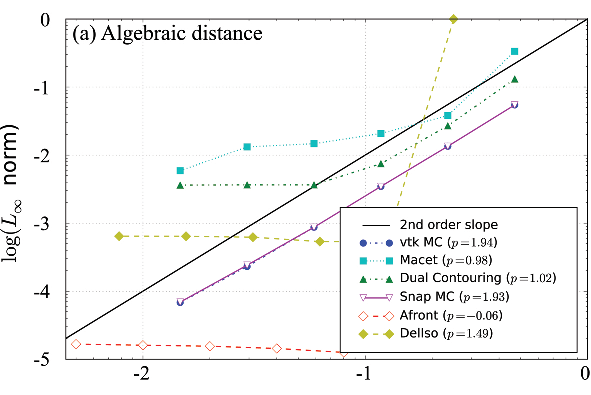
\includegraphics[width=0.48\linewidth,keepaspectratio=true]{chapter2/figures/all_meshconv-bug.pdf}}
\subfigure{
\label{fig:normconver}
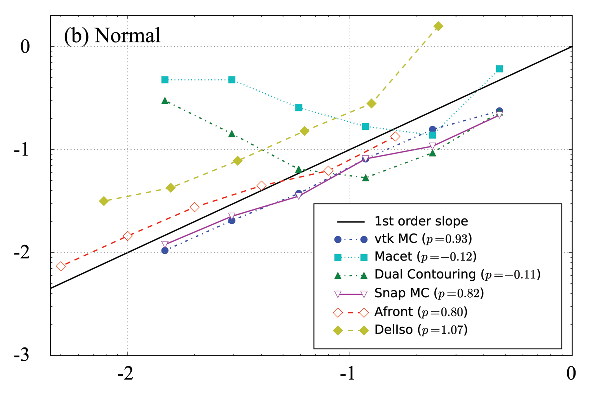
\includegraphics[width=0.48\linewidth,keepaspectratio=true]{chapter2/figures/all_normalconv-bug.pdf}}
\subfigure{
\label{fig:areaconv}
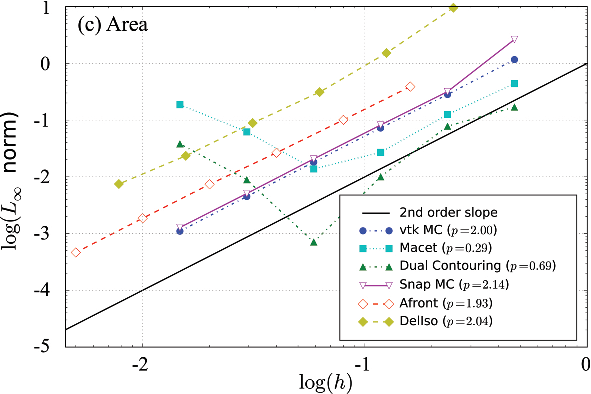
\includegraphics[width=0.48\linewidth,keepaspectratio=true]{chapter2/figures/all_areaconv-bug.pdf}}
\subfigure{
\label{fig:curvatureconv}
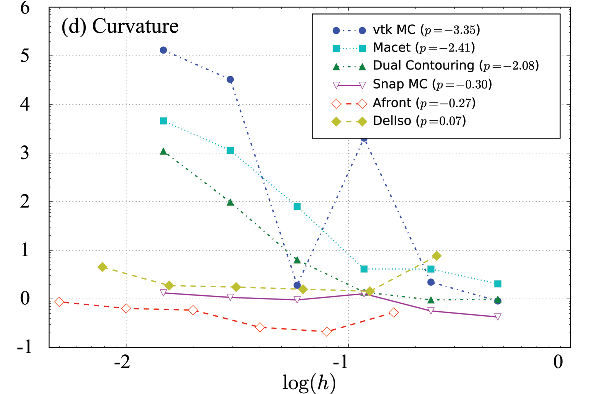
\includegraphics[width=0.48\linewidth,keepaspectratio=true]{chapter2/figures/all_curvconv-bug.pdf}}
\caption{Observed order of accuracy. The implementations of 
Macet and Dual Contouring have a bug that causes the deviation on errors. The black 
continuous line represents the expected behavior. $p$ is the slope of the linear 
regression for each curve.}
\end{figure}
\end{landscape}

\begin{landscape}
\begin{figure}
\centering
\subfigure{
\label{fig:meshconver-fixed}
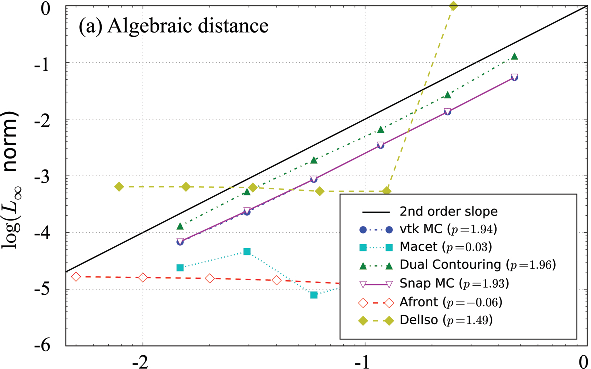
\includegraphics[width=0.487\linewidth,keepaspectratio=true]{chapter2/figures/all_meshconv.pdf}}
\subfigure{
\label{fig:normconver-fixed}
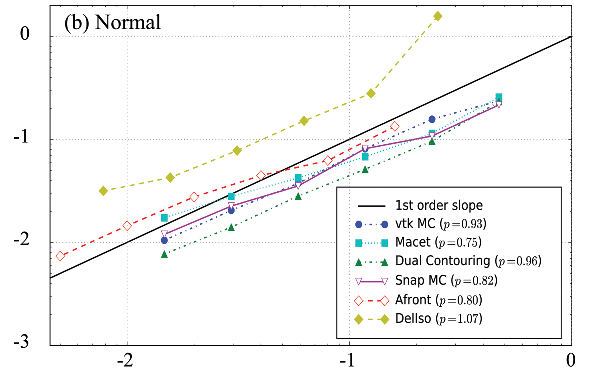
\includegraphics[width=0.488\linewidth,keepaspectratio=true]{chapter2/figures/all_normalconv.pdf}}
\subfigure{
\label{fig:areaconv-fixed}
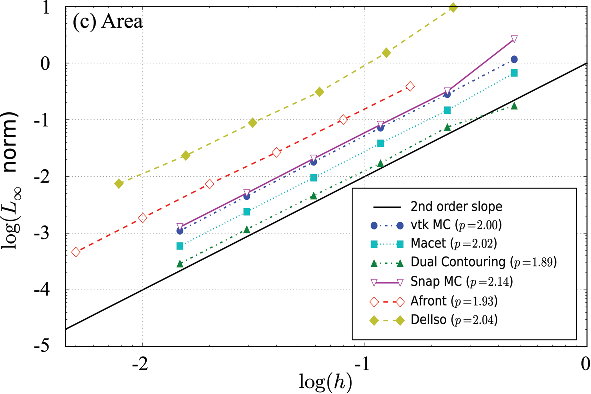
\includegraphics[width=0.49\linewidth,keepaspectratio=true]{chapter2/figures/all_areaconv.pdf}}
\subfigure{
\label{fig:curvatureconv-fixed}
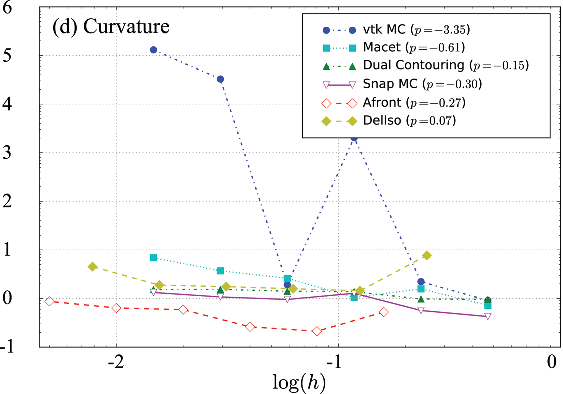
\includegraphics[width=0.485\linewidth,keepaspectratio=true]{chapter2/figures/all_curvconv.pdf}}
\caption{Observed order of accuracy after fixing Macet and Dual Contouring code (other curves remain the same). The black continuous line represents the expected behavior. $p$ is the slope of the linear regression for each curve.}
\label{fig:allconv-fixed}
\end{figure}
\end{landscape}

\subsubsection{Normals}
\label{subchap1:sec:normal-convergence}

Section \ref{chap1:sec:normalconvergence} shows that 
one expects first-order of accuracy for normal computations. 
We define the following approximation error using $L_\infty$ norm:
\begin{equation}
E_{k} = \max_{j=1\cdots n}|\theta_{\sigma_j}|
\label{eq:normerror}
\end{equation}
where $\theta_{\sigma_j}$ is the angle between the normal of 
the triangle $\sigma_j$ and the normal of 
the point in $S$ closest to the centroid of $\sigma_j$.
As shown in Figure \ref{fig:normconver}, VTK Marching Cubes, Afront,
SnapMC, and DelIso have good observed order of accuracy above $0.8$. However, only 
VTK Marching Cubes and DelIso present close proximity to linear. 
Macet and Dual Contouring once again do not present a consistent order. 
Figure \ref{fig:normconver-fixed} shows the results after fixing both codes.

\subsubsection{Area}
\label{chap1:sec:area-observed-order-of-accuracy}

Although there is no formal order of accuracy for area, one expects \emph{some}
convergence for it (Section \ref{chap1:sec:areaconvergence}).
We define the following approximation error:
\begin{equation}
E_{k} = |A(S) - A(\tilde{S}_k)|
\label{eq:surfareaerror}
\end{equation}
where $A$ is the area function of a continuous or piecewise-linear surface. 
The results are shown in Figure~\ref{fig:areaconv}. 
VTK Marching Cubes, Afront, and DelIso present second-order of accuracy, as shown 
in Figure \ref{fig:areaconv}. SnapMC accuracy is slightly better than quadratic due 
to poor approximation for large $h$. The error dropped faster than quadratic when the 
grid was refined for the first time. Macet and Dual Contouring exhibit once again  
unexpected behavior. Unlike the previous time, the curves now seem to diverge 
when $h$ is too small. Once the bug is fixed, the convergence curves changes,
and they become quadratic (Figure \ref{fig:areaconv-fixed}).
 
\subsubsection{Curvature}

Section \ref{chap1:sec:curvconvergence} shows that one expects zero-th order of accuracy for 
curvature computation. 
We define the approximation error using $L_\infty$ norm:
\begin{equation}
E_{k} = \max_{j=1\cdots n}|K(v_j) - \tilde{K}(v_j)|
\label{eq:curverror}
\end{equation}
where $K(v)$ is the Gaussian curvature at $v \in S$ and $\tilde{K}(v)$ is the Gaussian curvature at $v \in \tilde{S}$. In this
particular case where $S$ is a sphere, $K(v) = 1$ for every $v \in S$. The results 
are shown in Figure~\ref{fig:curvatureconv}.
DelIso, Afront, and SnapMC are close to zeroth-order accuracy. The
curvature order of accuracy for VTK Marching Cubes, on the other hand,
diverges significantly. This unexpected behavior might deserve further
investigation which we leave for future work.
Although the curves shown in Figure~\ref{fig:curvatureconv} for Macet and 
Dual Contouring diverge, they change after fixing the code 
(Figure \ref{fig:curvatureconv-fixed}).

\subsection{Detected Bugs}

We were able to find and fix bugs in two of the implementations 
under verification, namely, Macet and Dual Contouring, using as  
manufactured solution a sphere centered at origin with radius $1$. 
The new result curves are shown in Figure \ref{fig:allconv-fixed}. The observed 
order of accuracy for Dual Contouring is quite satisfactory for all manufactured 
solution. In particular, the normal order of accuracy has the best rate among the 
methods. Macet improved for its results for area. On the other hand, it still has 
some issues related to normals, which perhaps indicates a need for more tests 
and verification. The new order of accuracy for algebraic 
distance (Figure \ref{fig:meshconver-fixed}) does not tell us 
much about the correctness of the code because of the zero-th order 
of accuracy (same for Afront). 

The zero-th order of accuracy might happen if the formal order of accuracy 
is zero-th order, in which case the observed order matches the formal order. 
It might also happen due to a poor choice for manufactured solution. If 
it is not complex enough, the implementation being tested may approximate 
exactly the solution and therefore there is no error within the approximation 
although another error source (truncation error, for instance) may show up. 
The next section presents a detailed discussion concerning MMS.

Although we managed to fix the Macet convergence problem, we were not 
able to do so in a way that preserves triangle quality.
Two were the problems we found in the source code, and we proposed two 
solutions for one of them. Table \ref{tab:results-macet} shows that we could 
not find any combination that both fixed the convergence problem and preserved the 
triangle quality simultaneously. This sort of behavior raises the question if there 
is a theoretical problem that prevents both from being satisfied simultaneously, 
or it is just a matter of finding a better algorithmic fix. 
In both cases, further study and subsequent tests must be accomplished.

%\begin{landscape}
%\begin{figure}
%\centering
%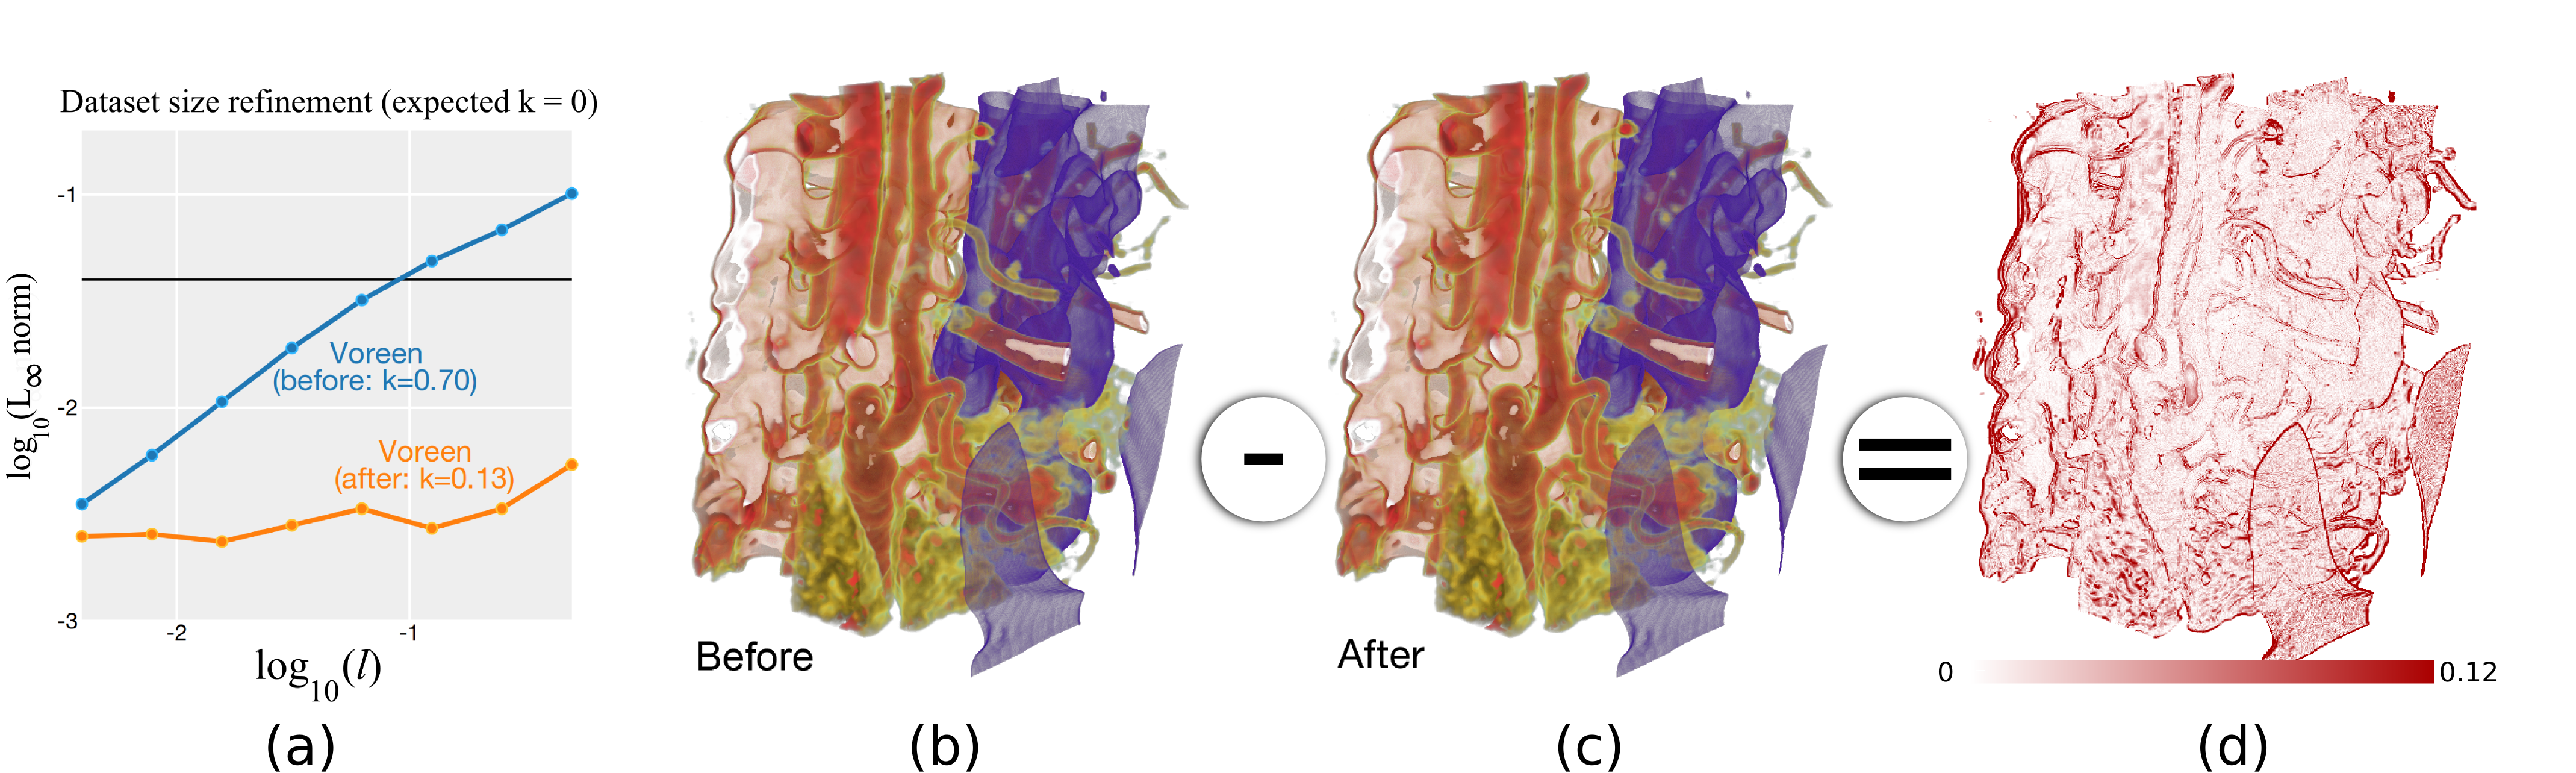
\includegraphics[width=1\linewidth]{chapter2/figures/teaser.pdf}
%\caption{Through the verification methodology presented on this chapter, 
%we were able to uncover a convergence problem within a publicly available marching-based 
%isosurfacing code (top left) and fix it (top right). The problem causes the mesh normals to 
%\emph{disagree} with the known gradient field when refining the voxel size $h$ (bottom row). 
%The two graphs show the convergence of the normals before and after fixing the code.}
%\label{fig:teaser}
%\end{figure}
%\end{landscape}

\begin{table}[t]
\caption{Table of results for Macet. Triangle quality versus 
convergence. We were not able to find a solution that provides 
both triangle quality and convergence.}
\centering
\begin{tabular}{cccc}
Bug $\#1$ & Bug $\#2$ & Quality & Observed accuracy \\
\hline
No Fix & No Fix & Good & Bad  \\
\hline
Fix 1 & No Fix & Good & Bad\\
Fix 1 & Fixed & Bad & Good\\
\hline
Fix 2 & No Fix & Good & Bad\\
Fix 2 & Fixed & Bad & Good\\
\hline
\end{tabular}
\label{tab:results-macet}
\end{table}